\documentclass{beamer}

\usepackage{amsmath, amssymb, graphicx, multicol, tikz, array}
\usepackage[absolute,overlay]{textpos}
\usepackage[export]{adjustbox}
\usepackage{pgfplots, pgf-pie}
\usetikzlibrary{positioning}
\usetikzlibrary{calc}
\pgfplotsset{compat=1.17}

% \usepackage{zxjatype}
% \usepackage[ipa]{zxjafont}
% \usepackage{mymacro}

\setbeamerfont*{itemize/enumerate body}{size=\large}
\setbeamerfont*{itemize/enumerate subbody}{parent=itemize/enumerate body}
\setbeamerfont*{itemize/enumerate subsubbody}{parent=itemize/enumerate body}

\usefonttheme{professionalfonts}
\setbeamertemplate{navigation symbols}{}

% --- page number ---
\setbeamertemplate{footline}{%
	\raisebox{10pt}{\makebox[\paperwidth]{\hfill\makebox[7em]{\normalsize\texttt{\insertframenumber/\inserttotalframenumber}}}}%
}

\DeclareMathOperator*{\argmin}{argmin}
\DeclareMathOperator*{\argmax}{argmax}
\DeclareMathOperator{\softmax}{softmax}
\DeclareMathOperator{\ReLU}{ReLU}

\title{Deep learning}
\subtitle{Part 1: Neural networks}
\author{Matthew Greenberg}
\date{2021.05.03}


\begin{document}

    \begin{frame}
    \maketitle
    \end{frame}

    \begin{frame}
        \frametitle{This course}
    
        \begin{enumerate}
            \setlength\itemsep{1em}
            \item Introduction
            
            \item Convolutional neural networks (CNNs) for computer vision
            
            \item Text processing and recurrent neural networks (RNNs)
        \end{enumerate}
    
    \end{frame}

    \begin{frame}
        \frametitle{Artificial intelligence (AI)}

        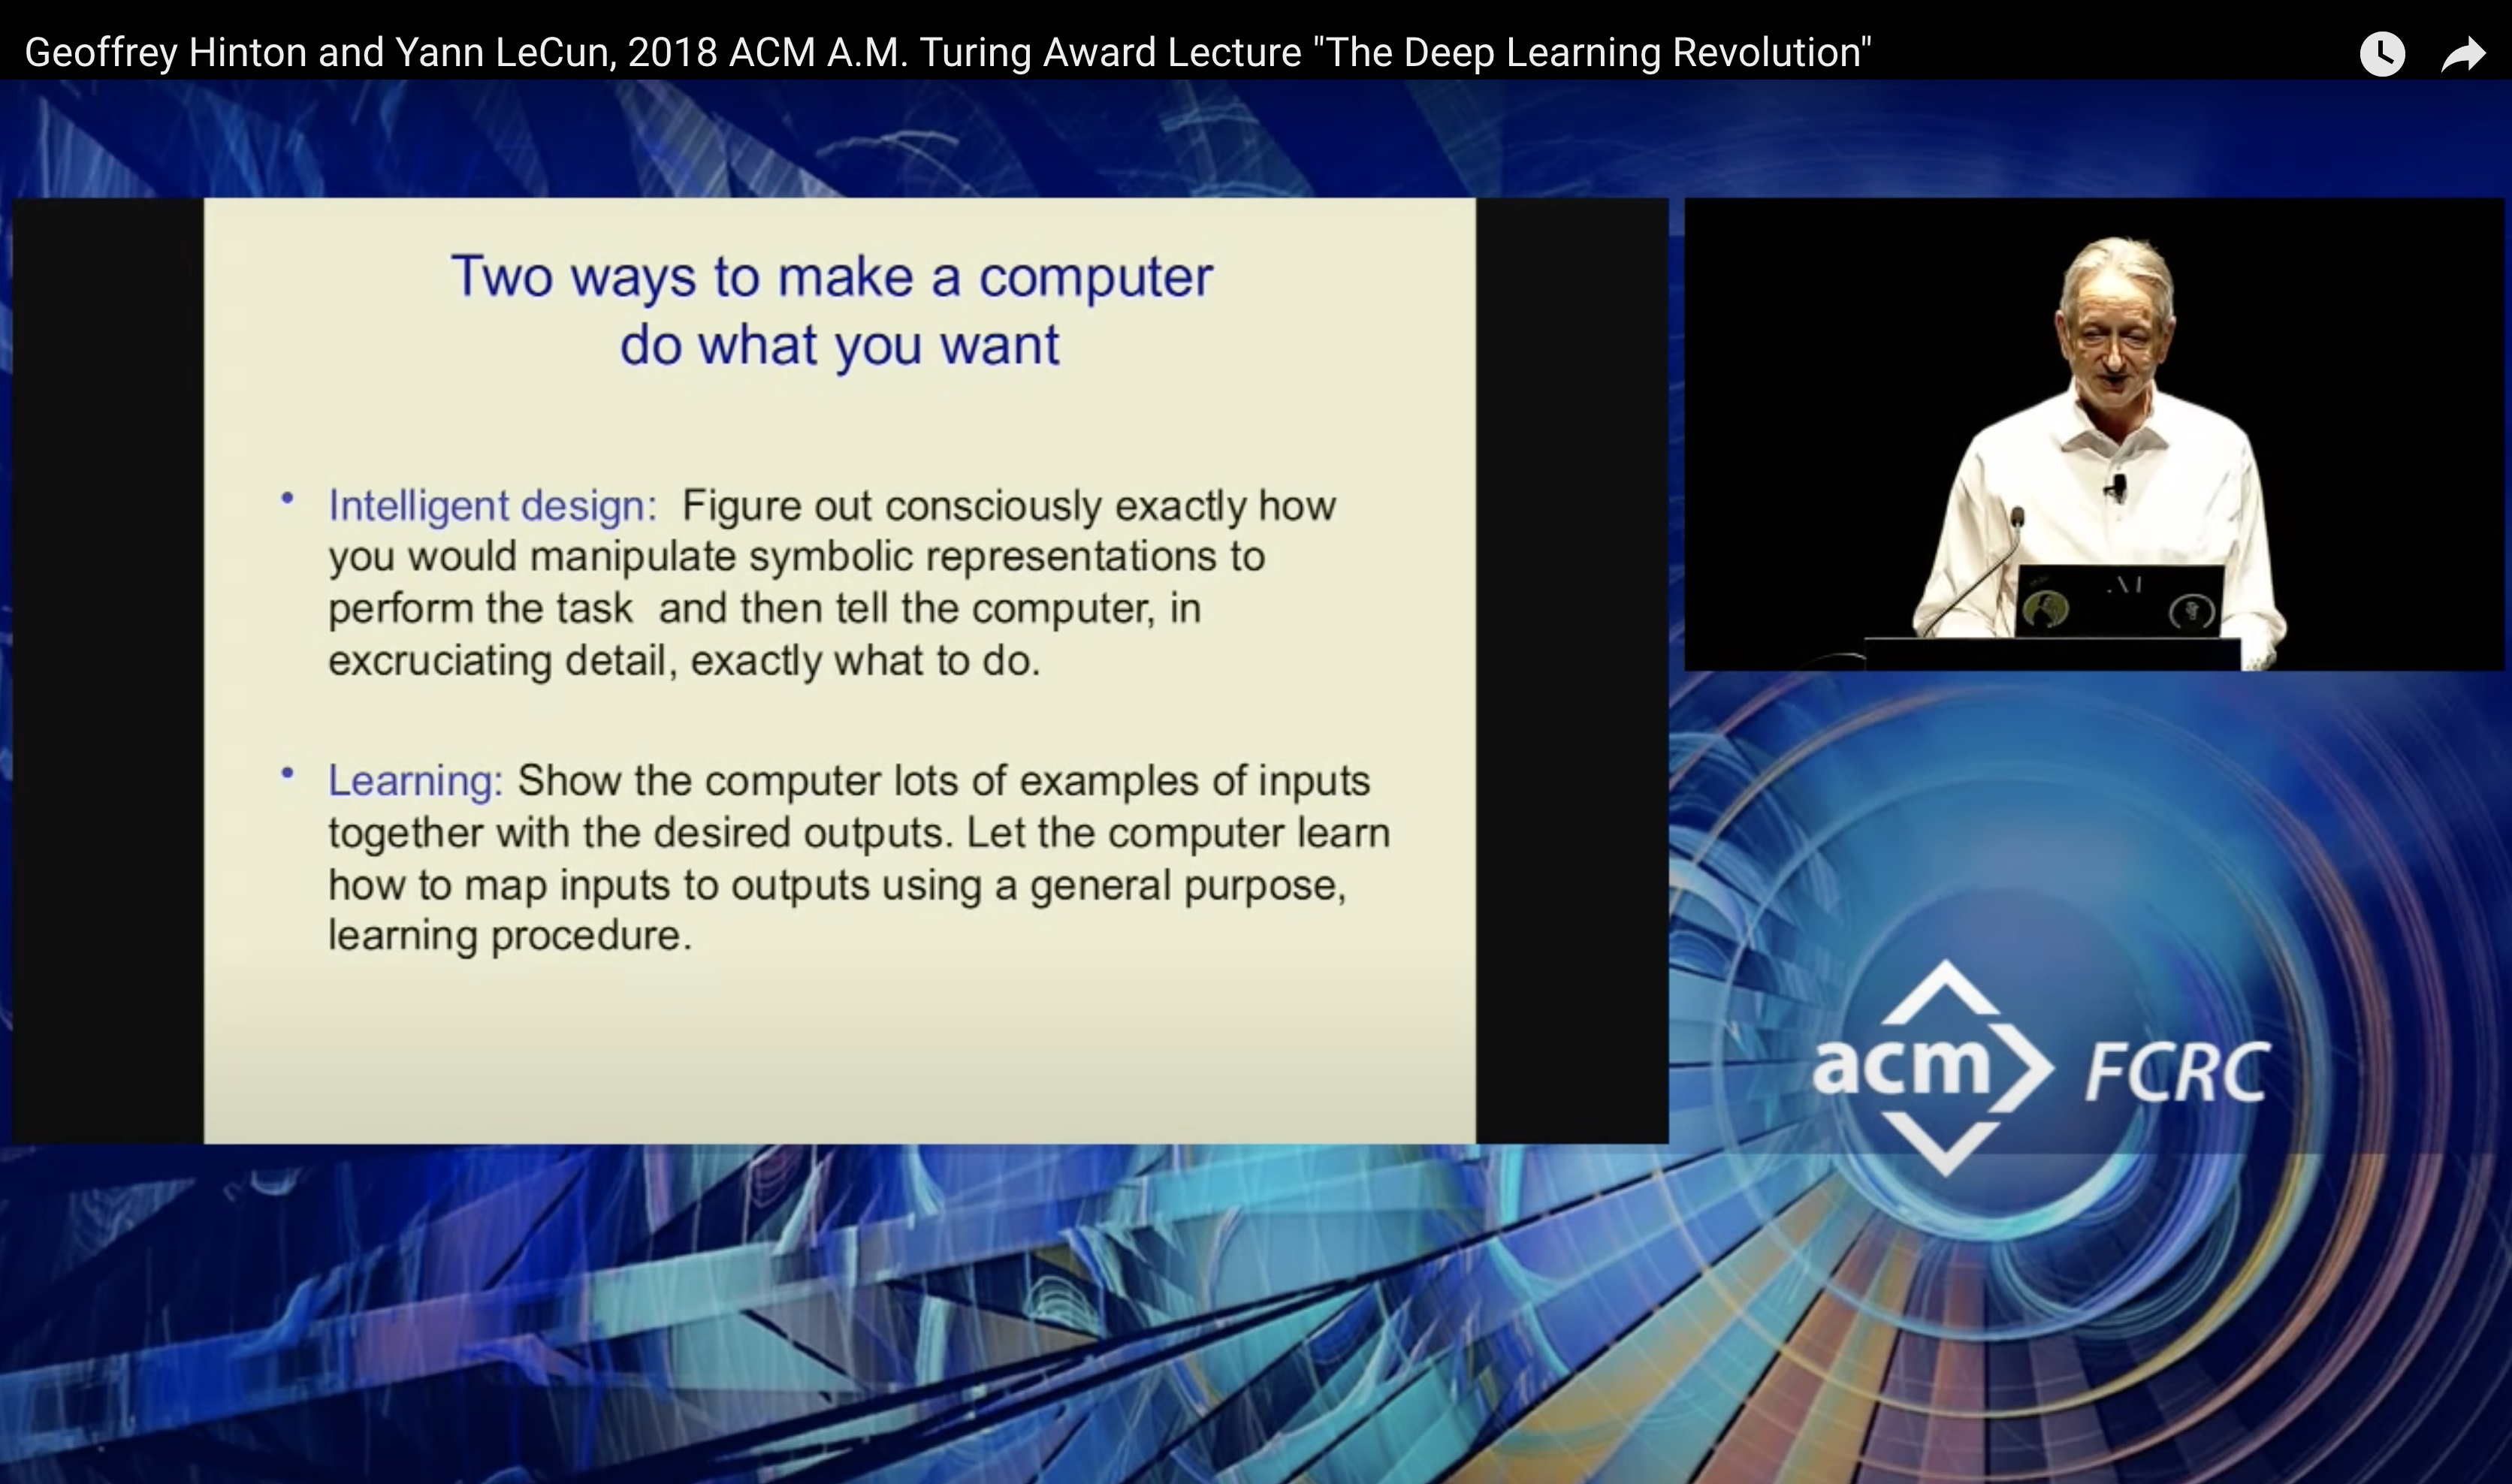
\includegraphics[width=\textwidth]{hinton-two-ways.jpg}

        \texttt{https://www.youtube.com/watch?v=VsnQf7exv5I} (11:49)
    \end{frame}

    \begin{frame}
        \frametitle{Machine learning (ML)}

        \bigskip
        \begin{quote}
            Show the computer lots of examples of inputs together with the desired outputs.
            Let the computer learn how to map inputs to outputs using a general purpose learning procedure.
        \end{quote}

        \bigskip
        \begin{tabular}{ m{0.75in} m{0.5in} || m{1in} m{1.25in} }
            \textbf{input}&\textbf{output}&\textbf{input}&\textbf{output}\\[0.5em]
            \textit{image}&\textit{label}&\textit{English text}&\textit{French translation}\\[0.5em]
            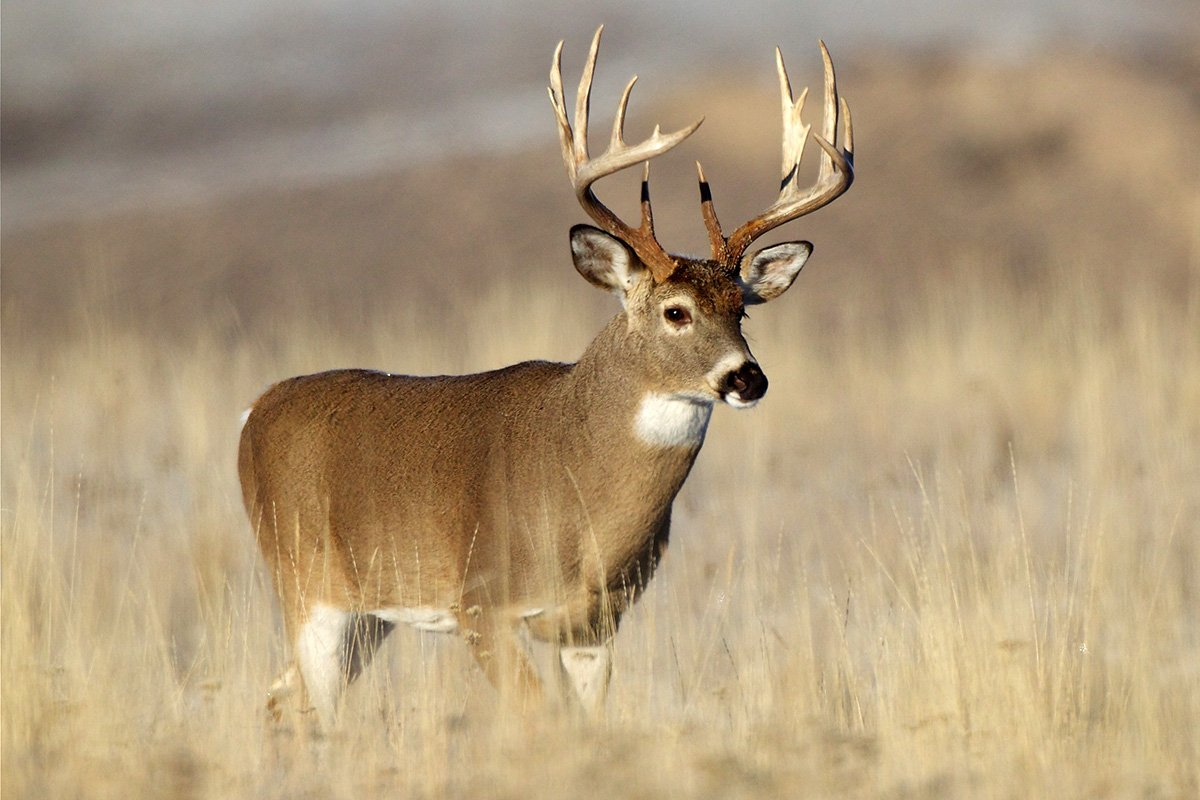
\includegraphics[width=0.75in]{deer.jpg}&deer&\footnotesize Can I borrow your magazine?&\footnotesize Puis-je emprunter votre magazine?\\
            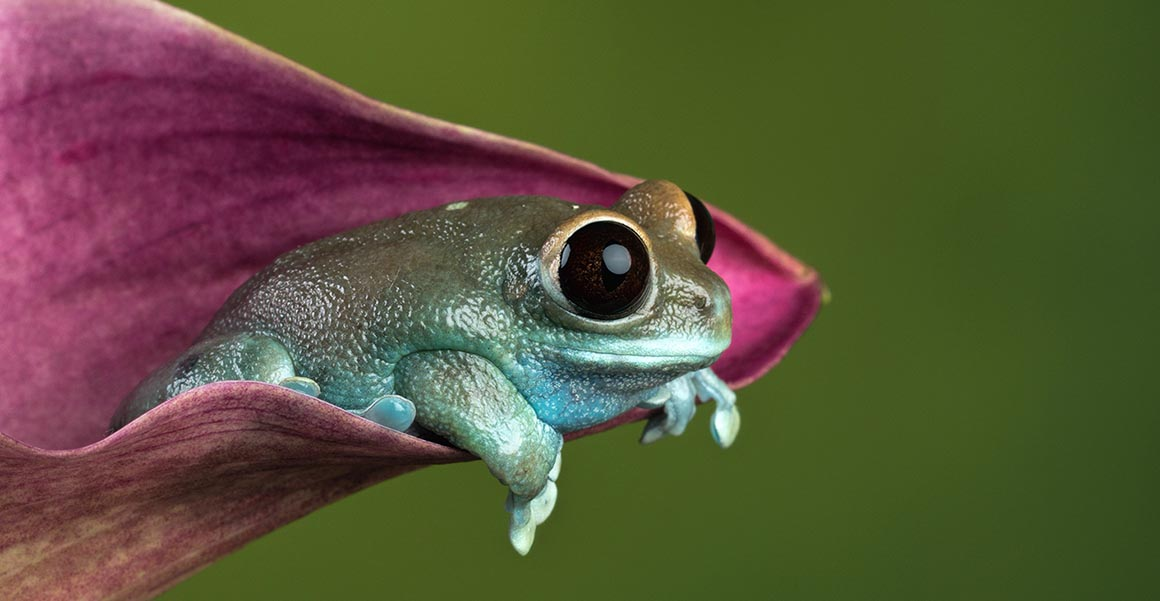
\includegraphics[width=0.75in]{frog.jpg}&frog&\footnotesize Please pass the ketchup.&\footnotesize Veuillez passer le ketchup.\\
            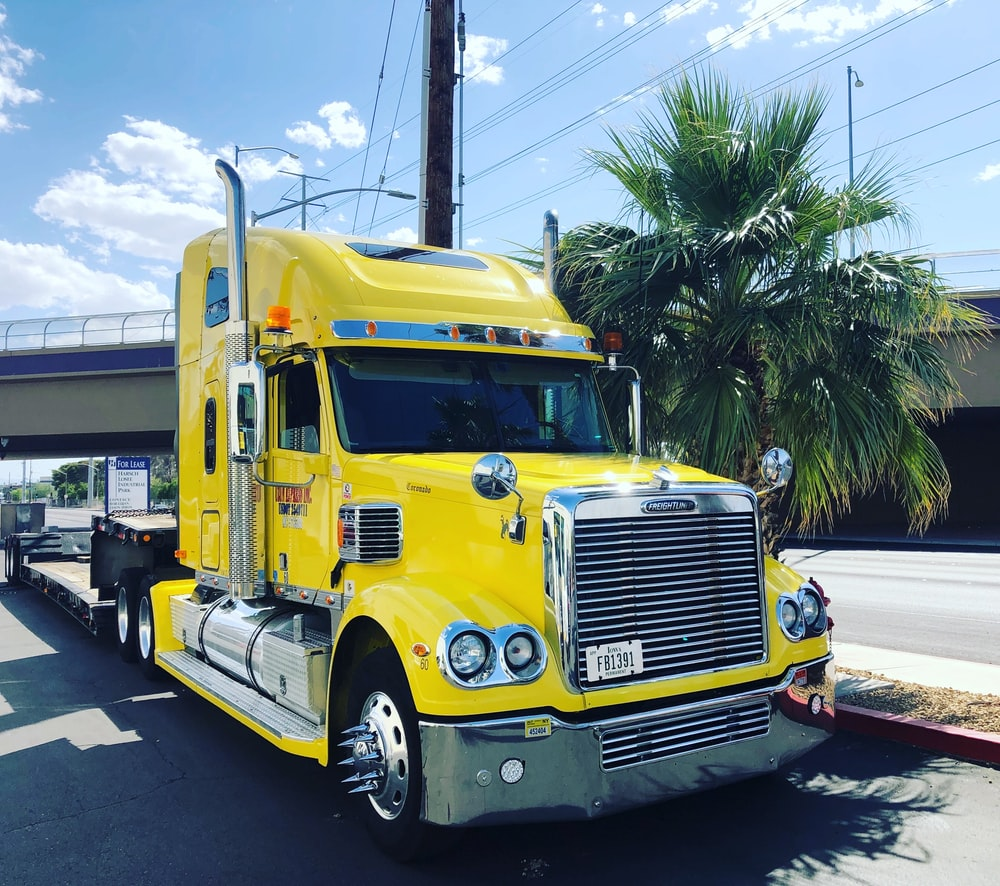
\includegraphics[width=0.75in]{truck.jpg}&truck&\footnotesize His shirt was made in turkey.&\footnotesize Sa chemise a \'et\'e confectionnée en Turquie.\\
        \end{tabular}
    \end{frame}
    
    

    

    \begin{frame}
        \frametitle{Deep learning (DL)}

        \begin{center}
        
\includegraphics[scale=0.35]{lecundef.png}
        \end{center}
    \end{frame}

    \begin{frame}
        \frametitle{Networks}
        \bigskip

        \textbf{Traditional machine learning}

        \bigskip
        \begin{tikzpicture}[
            redsquarednode/.style={rectangle, rounded corners, draw=red!60, fill=red!5, very thick},
            bluesquarednode/.style={rectangle, rounded corners, draw=blue!60, fill=blue!5, very thick},
            ]
            \node (frog) {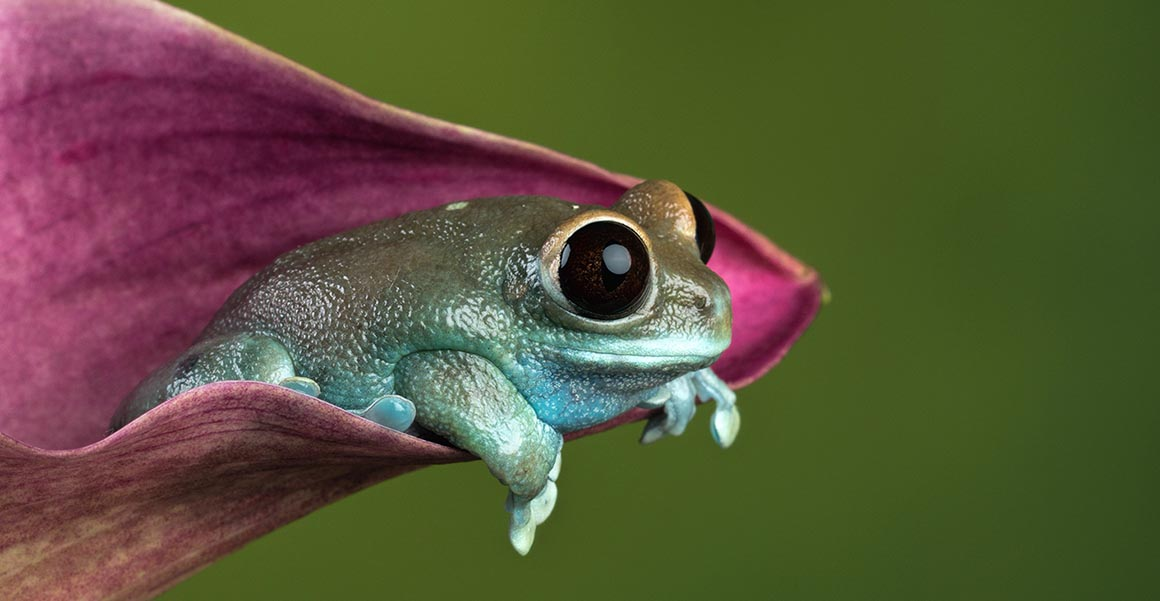
\includegraphics[width=1in]{frog.jpg}};

            \node[redsquarednode, align=center, right=of frog] (fe) {hand-engineered\\feature extractor};
            \node[bluesquarednode, align=center, right=of fe] (lc) {trainable\\classifier};
            \node[right=of lc] (yhat) {$\widehat{p}$};

            \draw[->, very thick] (frog.east) -- (fe.west);
            \draw[->, very thick] (fe.east) -- (lc.west);
            \draw[->, very thick] (lc.east) -- (yhat.west);
        \end{tikzpicture}


        \bigskip
        \textbf{Deep learning}

        \bigskip
        \begin{tikzpicture}[
            redsquarednode/.style={rectangle, rounded corners, draw=red!60, fill=red!5, very thick},
            greensquarednode/.style={rectangle, rounded corners, draw=green!60, fill=green!5, very thick},
            bluesquarednode/.style={rectangle, rounded corners, draw=blue!60, fill=blue!5, very thick},
            ]
            \node (frog) {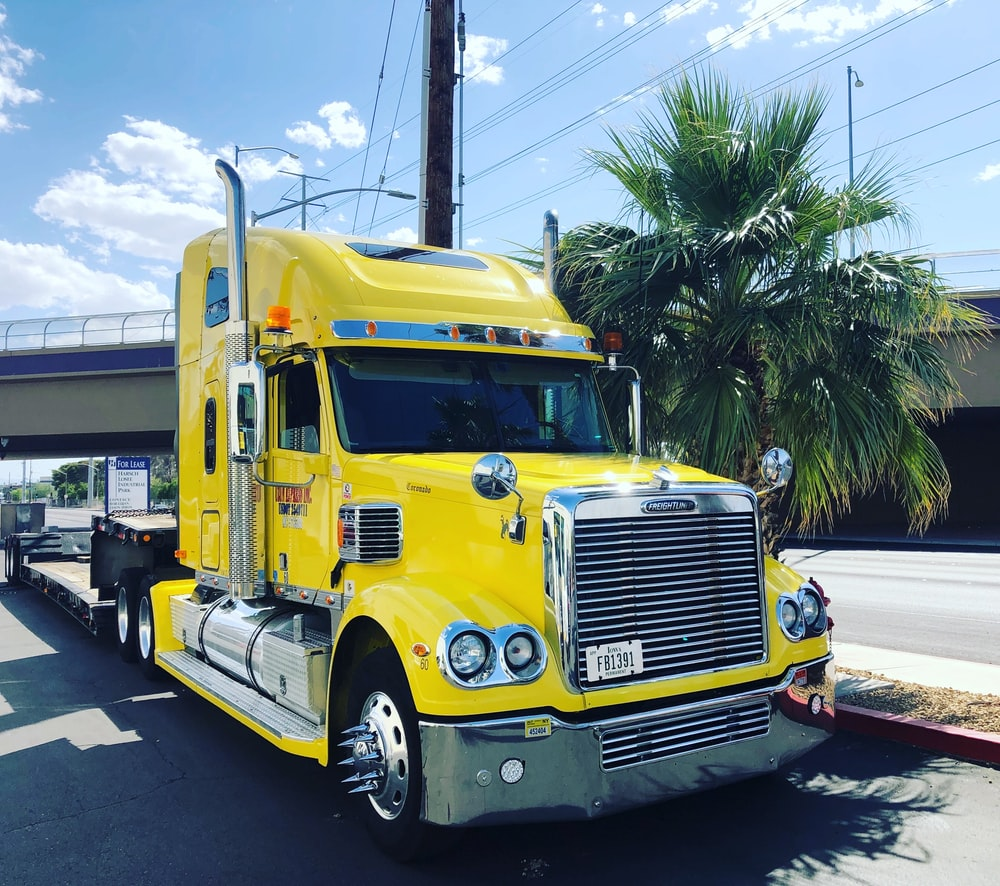
\includegraphics[width=1in]{truck.jpg}};

            \node[greensquarednode, align=center, right=of frog] (fe) {trainable\\feature extractor};
            \node[bluesquarednode, align=center, right=of fe] (lc) {trainable\\classifier};
            \node[right=of lc] (yhat) {$\widehat{p}$};

            \draw[->, very thick] (frog.east) -- (fe.west);
            \draw[->, very thick] (fe.east) -- (lc.west);
            \draw[->, very thick] (lc.east) -- (yhat.west);
        \end{tikzpicture}

        \bigskip
        \begin{itemize}
            \item $\hat{p}$ is a vector of class probabilities.
        \end{itemize}
    \end{frame}

    
    \begin{frame}
        \frametitle{Feature hierarchy}
    
        \begin{tikzpicture}[
            redsquarednode/.style={rectangle, rounded corners, draw=red!60, fill=red!5, very thick},
            greensquarednode/.style={rectangle, rounded corners, draw=green!60, fill=green!5, very thick},
            bluesquarednode/.style={rectangle, rounded corners, draw=blue!60, fill=blue!5, very thick},
            ]
            \node (deer) {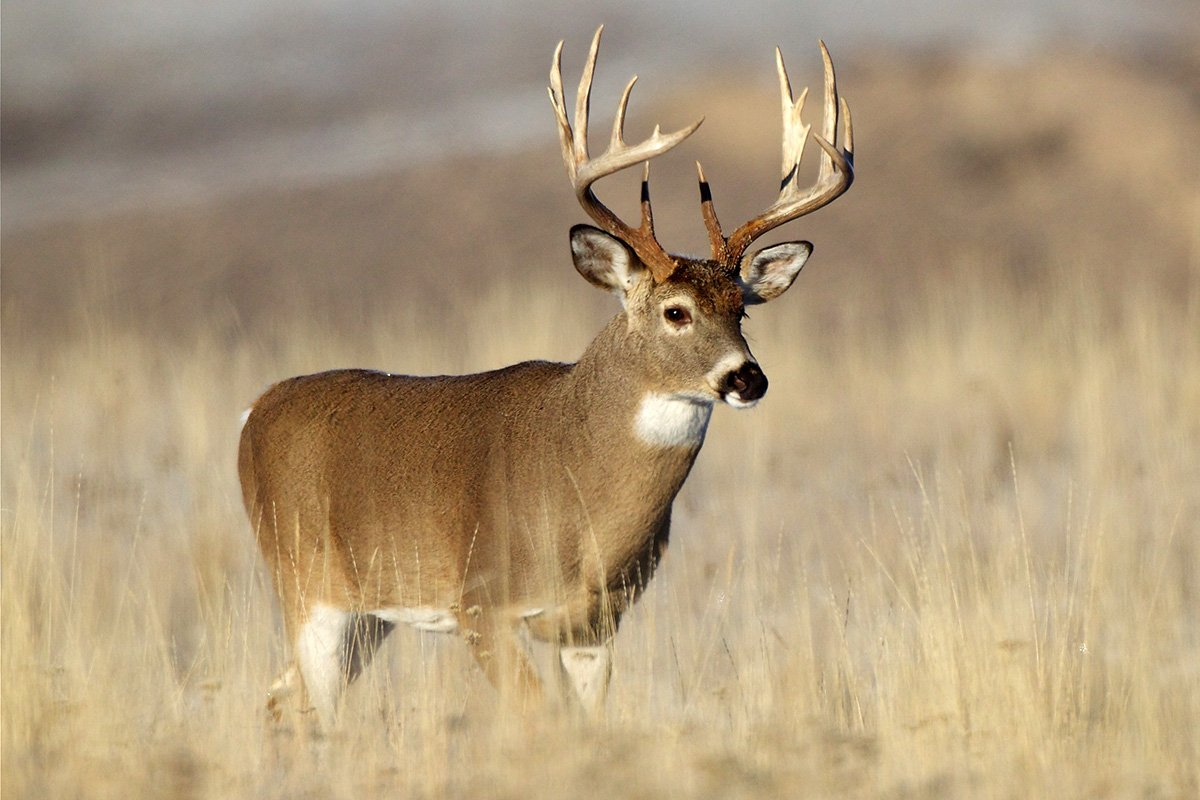
\includegraphics[width=1in]{deer.jpg}};

            \node[greensquarednode, align=center, below=of deer] (lowfe) {low-level\\feature extractor};
            \node[greensquarednode, align=center, right=of lowfe] (midfe) {mid-level\\feature extractor};
            \node[greensquarednode, align=center, right=of midfe] (highfe) {high-level\\feature extractor};
            \node[bluesquarednode, align=center, above=of highfe] (tc) {classifier};
            \node[above=of tc] (yhat) {$\widehat{p}$};
            \node[above=of midfe] (trainable) {\textit{trainable}};
            \node[below=of lowfe, magenta] {\textit{patterns of pixels}};
            \node[below=of midfe, align=center, magenta] {\textit{patterns of patterns}};
            \node[below=of highfe, align=center, magenta] {\textit{patterns of patterns}\\\textit{of patterns}};

            \draw[->, very thick] (deer.south) -- (lowfe.north);
            \draw[->, very thick] (lowfe.east) -- (midfe.west);
            \draw[->, very thick] (midfe.east) -- (highfe.west);
            \draw[->, very thick] (highfe.north) -- (tc.south);
            \draw[->, very thick] (tc.north) -- (yhat.south);
            \draw[dashed] (trainable.east) -- (tc.west);
            \draw[dashed] (trainable.south east) -- (highfe.north west);
            \draw[dashed] (trainable.south) -- (midfe.north);
            \draw[dashed] (trainable.south west) -- (lowfe.north east);
        \end{tikzpicture}
    \end{frame}

    \begin{frame}
        \frametitle{Linear layers}

        \bigskip
        Trainable parameters:

        \bigskip
        \begin{itemize}
            \setlength\itemsep{1em}
            \item \textbf{weights:} $W\in\mathbb{R}^{p\times q}$
            \item \textbf{biases:} $b\in\mathbb{R}^q$
        \end{itemize}
        
        \bigskip
        \begin{center}
            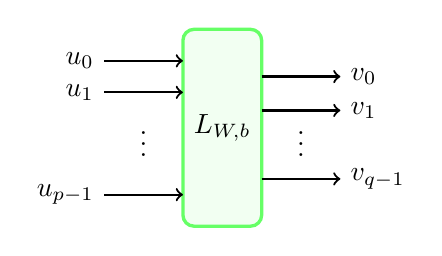
\begin{tikzpicture}
                \draw[rounded corners, draw=green!60, fill=green!5, very thick] (2,0) rectangle (3, 2.5);
    
                \draw[thick, ->] (1,0.4) node[anchor=east] {$u_{p-1}$} -- (2,0.4);
                \draw[thick, ->] (1,1.7) node[anchor=east] {$u_1$} -- (2,1.7);
                \draw[thick, ->] (1,2.1) node[anchor=east] {$u_0$} -- (2,2.1);
                \draw (1.5, 1.15) node {$\vdots$};
            
                \draw[thick, ->] (3,{0.6}) -- (4,{0.6}) node[anchor=west] {$v_{q-1}$};
                \draw[thick, ->] (3,{1.9 - 0.43}) -- (4,{1.9 - 0.43}) node[anchor=west] {$v_1$};
                \draw[thick, ->] (3,{1.9}) -- (4,{1.9}) node[anchor=west] {$v_0$};
                \draw (3.5, 1.15) node {$\vdots$};
            
                \draw (2.5, 1.25) node {$L_{W,b}$};
            \end{tikzpicture}
        \end{center}

        More concisely:
    \begin{center}
        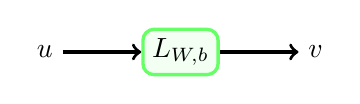
\begin{tikzpicture}[
            redsquarednode/.style={rectangle, rounded corners, draw=red!60, fill=red!5, very thick},
            greensquarednode/.style={rectangle, rounded corners, draw=green!60, fill=green!5, very thick},
            bluesquarednode/.style={rectangle, rounded corners, draw=blue!60, fill=blue!5, very thick},
            ]
            \node (input) {$u$};
            \node[greensquarednode, right=of input] (L) {$L_{W,b}$};
            \node[right=of L] (output) {$v$};
            \draw[->, very thick] (input.east) -- (L.west);
            \draw[->, very thick] (L.east) -- (output.west);
        \end{tikzpicture}
    \end{center}

        \[
            v = L_{W,b}(u) = uW + b
        \]
    \end{frame}

    \begin{frame}
        \frametitle{Compositions of linear layers are linear}
    
        \bigskip
        \begin{center}
        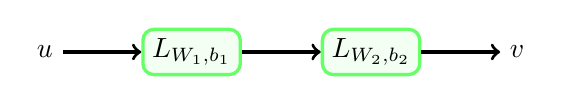
\begin{tikzpicture}[
            redsquarednode/.style={rectangle, rounded corners, draw=red!60, fill=red!5, very thick},
            greensquarednode/.style={rectangle, rounded corners, draw=green!60, fill=green!5, very thick},
            bluesquarednode/.style={rectangle, rounded corners, draw=blue!60, fill=blue!5, very thick},
            ]

            \node (input) {$u$};
            \node[greensquarednode, right=of input] (L1) {$L_{W_1,b_1}$};
            \node[greensquarednode, right=of L1] (L2) {$L_{W_2,b_2}$};
            \node[right=of L2] (output) {$v$};

            \draw[->, very thick] (input.east) -- (L1.west);
            \draw[->, very thick] (L1.east) -- (L2.west);
            \draw[->, very thick] (L2.east) -- (output.west);
        \end{tikzpicture}
    \end{center}
    
    \begin{align*}
        L_{W_2,b_2}\big(L_{W_1, b_1}(u)\big) &= L_{W_2,b_2}(uW_1 + b_1)\\[0.25em]
        &= (uW_1+b_1)W_2 + b_2\\[0.25em]
        &= u\underbrace{W_1W_2}_{W} + \underbrace{b_1W_2 + b_2}_{b}\\
        &= L_{W,b}(u)
    \end{align*}

    \bigskip
    \begin{center}
        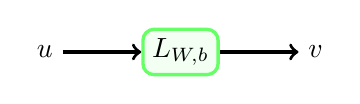
\begin{tikzpicture}[
            redsquarednode/.style={rectangle, rounded corners, draw=red!60, fill=red!5, very thick},
            greensquarednode/.style={rectangle, rounded corners, draw=green!60, fill=green!5, very thick},
            bluesquarednode/.style={rectangle, rounded corners, draw=blue!60, fill=blue!5, very thick},
            ]
            \node (input) {$u$};
            \node[greensquarednode, right=of input] (L) {$L_{W,b}$};
            \node[right=of L] (output) {$v$};
            \draw[->, very thick] (input.east) -- (L.west);
            \draw[->, very thick] (L.east) -- (output.west);
        \end{tikzpicture}
    \end{center}
    \end{frame}


    \begin{frame}
        \frametitle{$\ReLU$-activated linear layers}
    
        \begin{columns}
            \begin{column}{0.35\textwidth}
                Rectified linear unit:
        \[
            \ReLU(x) = \max(x, 0)
        \]
            \end{column}
            \begin{column}{0.65\textwidth}
                \bigskip

            \pgfplotsset{width=3in, height=1.75in}
            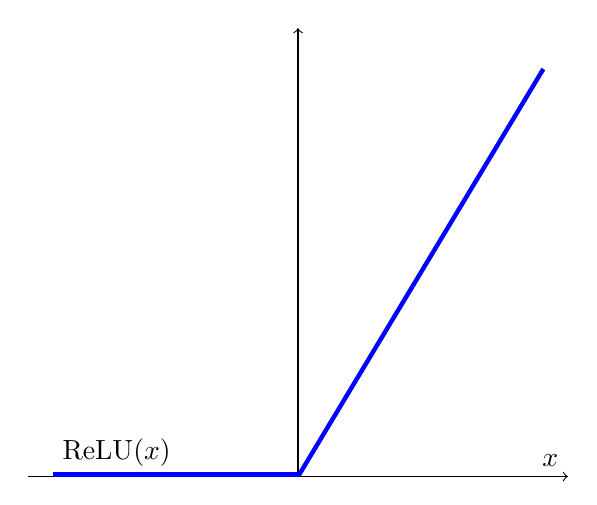
\begin{tikzpicture}
                \begin{axis}[
                    domain=0:1,
                    xmin=-1.1,
                    xmax=1.1,
                    ymin=0,
                    ymax=1.1,
                    ticks=none,
                    samples=1000,
                    axis lines=middle,
                    axis line style={->},
                    xlabel={$x$}
                    ]
                  \addplot[blue, ultra thick] (x,x);
                  \addplot[blue, line width=3pt] (-x,0) node[pos=1] (E) {};
                  \node[above right] at (E) {$\ReLU(x)$};
                \end{axis}
            \end{tikzpicture}
        \end{column}
    \end{columns}
    
    \bigskip
    \begin{center}
        \begin{tikzpicture}[
            orangesquarednode/.style={rectangle, rounded corners, draw=orange!60, fill=orange!5, very thick},
            greensquarednode/.style={rectangle, rounded corners, draw=green!60, fill=green!5, very thick},
            bluesquarednode/.style={rectangle, rounded corners, draw=blue!60, fill=blue!5, very thick},
            ]

            \node (input) {$u$};
            \node[greensquarednode, right=of input] (L) {$L_{W,b}$};
            \node[orangesquarednode, right=of L] (ReLU) {$\ReLU$};
            \node[right=of L2] (output) {$v$};
            

            \draw[->, very thick] (input.east) -- (L.west);
            \draw[->, very thick] (L.east) -- (ReLU.west);
            \draw[->, very thick] (ReLU.east) -- (output.west);

            \draw[rounded corners, ultra thick, magenta] ($(L.north west) + (-0.5, 0.7)$) rectangle ($(ReLU.south east) + (0.5, -0.9)$);
            \node at ($(ReLU.south) + (0.3, -0.5)$) {\Large$R_{W,b}$};
        \end{tikzpicture}
    \end{center}
    
    \[
        R_{W,b}(u) = \ReLU\big(L_{W,b}(u)\big)\qquad
        \text{(apply $\ReLU$ componentwise)}
    \]
    \end{frame}

    \begin{frame}
        \frametitle{A simple classification network}
    
        \begin{center}
        \begin{tikzpicture}[
            orangesquarednode/.style={rectangle, rounded corners, draw=orange!60, fill=orange!5, very thick},
            magentasquarednode/.style={rectangle, rounded corners, draw=magenta!60, fill=magenta!5, very thick},
            bluesquarednode/.style={rectangle, rounded corners, draw=blue!60, fill=blue!5, very thick},
            ]
            \node (image) {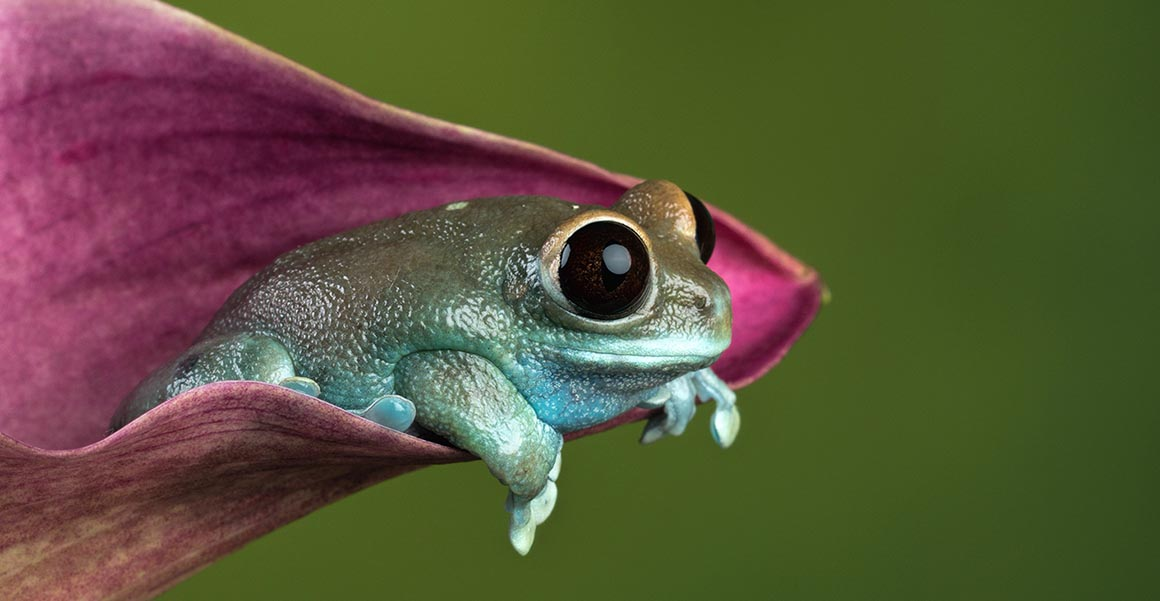
\includegraphics[width=1in]{frog.jpg}};
            \node[orangesquarednode, below=of image] (flatten) {flatten};
            \node[magentasquarednode, align=center, below=of flatten] (lowfe) {$R_{W_1, b_1}$};
            \node[magentasquarednode, align=center, right=of lowfe] (midfe) {$R_{W_2, b_2}$};
            \node[magentasquarednode, align=center, right=of midfe] (highfe) {$R_{W_3, b_3}$};
            \node[bluesquarednode, align=center, above=of highfe] (tc) {classifier};
            \node[above=of tc] (yhat) {$\widehat{p}$};
            \node[below=of midfe] (trainable) {\textit{hidden layers}};

            \draw[->, very thick] (image.south) -- (flatten.north);
            \draw[->, very thick] (flatten.south) -- (lowfe.north);
            \draw[->, very thick] (lowfe.east) -- (midfe.west);
            \draw[->, very thick] (midfe.east) -- (highfe.west);
            \draw[->, very thick] (highfe.north) -- (tc.south);
            \draw[->, very thick] (tc.north) -- (yhat.south);
            \draw[dashed] (trainable.north east) -- (highfe.south west);
            \draw[dashed] (trainable.north) -- (midfe.south);
            \draw[dashed] (trainable.north west) -- (lowfe.south east);
        \end{tikzpicture}
    \end{center}
    \begin{itemize}
        \item The \textbf{flatten} layer flattens an RGB image tensor with
        shape $m\times n\times c$ to an $mnc$-dimensional vector. 
    \end{itemize}
    \end{frame}

    \begin{frame}
        \frametitle{The classification layer: $\softmax$-activated linear layer}
    
        \begin{center}
            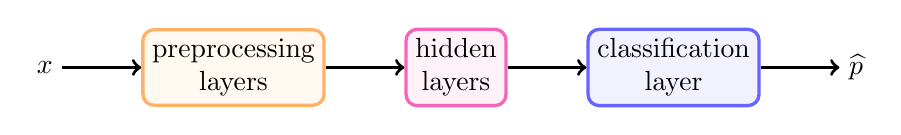
\begin{tikzpicture}[
                orangesquarednode/.style={rectangle, rounded corners, draw=orange!60, fill=orange!5, very thick},
                magentasquarednode/.style={rectangle, rounded corners, draw=magenta!60, fill=magenta!5, very thick},
                bluesquarednode/.style={rectangle, rounded corners, draw=blue!60, fill=blue!5, very thick},
                ]
                \node (input) {$x$};
                \node[orangesquarednode, align=center, right=of input] (pre) {preprocessing\\layers};
                \node[magentasquarednode, align=center, right=of pre] (hidden) {hidden\\layers};
                \node[bluesquarednode, align=center, right=of hidden] (class) {classification\\layer};
                \node[right=of class] (output) {$\widehat{p}$};
    
                \draw[->, very thick] (input.east) -- (pre.west);
                \draw[->, very thick] (pre.east) -- (hidden.west);
                \draw[->, very thick] (hidden.east) -- (class.west);
                \draw[->, very thick] (class.east) -- (output.west);
            \end{tikzpicture}
        \end{center}
    
        \begin{itemize}
            \item The classification layer of a $K$-class classification network typically performs \textbf{logistic regression}, mapping features output by the hidden layers onto class probabilities.
        \end{itemize}

        \begin{center}
            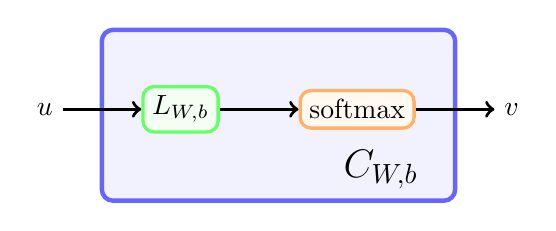
\begin{tikzpicture}[
                orangesquarednode/.style={rectangle, rounded corners, draw=orange!60, fill=orange!5, very thick},
                greensquarednode/.style={rectangle, rounded corners, draw=green!60, fill=green!5, very thick},
                bluesquarednode/.style={rectangle, rounded corners, draw=blue!60, fill=blue!5, very thick},
                ]
    
                \node (input) {$u$};
                \node[greensquarednode, right=of input] (L) {$L_{W,b}$};
                \node[orangesquarednode, right=of L] (ss) {$\softmax$};
                \node[right=of ss] (output) {$v$};
    
                \draw[rounded corners, ultra thick, draw=blue!60, fill=blue!5]
                ($(L.north west) + (-0.5, 0.7)$) rectangle
                ($(ss.south east) + (0.5, -0.9)$);
                \node at ($(ss.south) + (0.3, -0.5)$) {\Large$C_{W,b}$};

                \node[greensquarednode, right=of input] {$L_{W,b}$};
                \node[orangesquarednode, right=of L] (s) {$\softmax$};
                \draw[->, very thick] (input.east) -- (L.west);
                \draw[->, very thick] (L.east) -- (s.west);
                \draw[->, very thick] (s.east) -- (output.west);
            \end{tikzpicture}
        \end{center}
    \end{frame}

    \begin{frame}
        \frametitle{The softmax function}
    
        \begin{itemize}
            \item 
        The \textbf{softmax function} converts ``raw scores'' $u_0,\ldots,u_{p-1}$ into a \textbf{distribution vector}, i.e. a vector with nonnegative components that sum to $1$:
        \[
            \softmax(u_0,\ldots,u_{p-1}) = \frac1{\sum_j e^{u_j}}\left(e^{u_0},\ldots,e^{u_{p-1}}\right)
        \]
    \end{itemize}
    \end{frame}

    \begin{frame}
        \frametitle{Using pretrained image classification models}

        \bigskip
\begin{itemize}
    \setlength\itemsep{1em}
    \item You can download many pretrained image classification models.
    \item Most are trained on the \textbf{ImageNet dataset}, with
    
    \bigskip
    \begin{itemize}
        \setlength\itemsep{1em}
        \item 1000 object classes,
        \item $> 1.2$ million training images
    \end{itemize}
    \end{itemize}

    \bigskip
    \begin{center}
        
\includegraphics[width=3in]{imagenet.png}
    \end{center}        
    
    \end{frame}


    \begin{frame}
        \frametitle{Example: the CIFAR-10 dataset}

        \begin{itemize}
            \item $60000$ RGB images, $32\times 32$ pixels
            \item 10 classes
        \end{itemize}
    
        \bigskip
        \begin{tabular}{ m{0.8in} m{1in} | m{0.75in} m{1in} }
            \textbf{label/class} & \textbf{examples}& \textbf{label/class}&\textbf{examples}\\[0.5em]
            0/airplane & 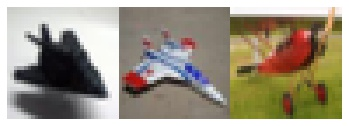
\includegraphics[width=1in]{../cifar10/airplane.jpg}&5/dog&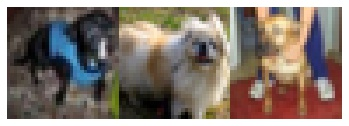
\includegraphics[width=1in]{../cifar10/dog.jpg}\\
            1/automobile & 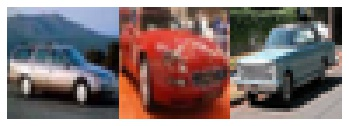
\includegraphics[width=1in]{../cifar10/automobile.jpg}&6/frog&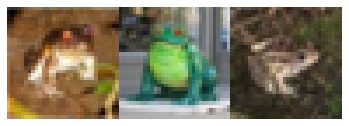
\includegraphics[width=1in]{../cifar10/frog.jpg}\\
            2/bird & 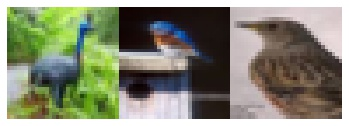
\includegraphics[width=1in]{../cifar10/bird.jpg}&7/horse&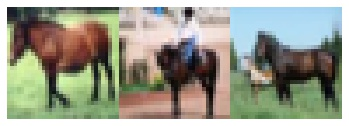
\includegraphics[width=1in]{../cifar10/horse.jpg}\\
            3/cat & 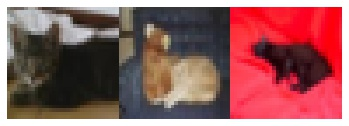
\includegraphics[width=1in]{../cifar10/cat.jpg}&8/ship&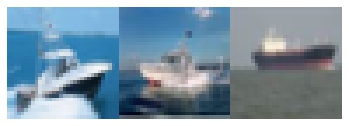
\includegraphics[width=1in]{../cifar10/ship.jpg}\\
            4/deer & 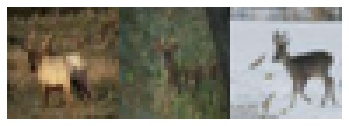
\includegraphics[width=1in]{../cifar10/deer.jpg}&9/truck&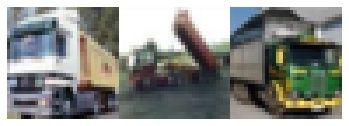
\includegraphics[width=1in]{../cifar10/truck.jpg}\\
        \end{tabular}
    \end{frame}

    \begin{frame}
        \frametitle{An image classifier for CIFAR-10}

        \begin{center}
            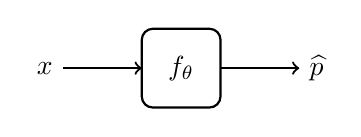
\begin{tikzpicture}
                \draw[rounded corners, thick] (2,0) rectangle (3, 1);
                \draw[thick, ->] (1,0.5) node[anchor=east] {$x$} -- (2,0.5);
                \draw[thick, ->] (3,0.5) -- (4,0.5) node[anchor=west] {$\widehat{p}$};
                \draw (2.5, 0.5) node {$f_\theta$};
            \end{tikzpicture}
        \end{center}

        \begin{itemize}
            \setlength\itemsep{1em}
            \item input $x$: tensor with shape $32\times32\times3$
            \item target: $y\in\{0,1,\ldots,9\}$
            \item output $\widehat{p}$: vector of length $10$, where
            \[
                \widehat{p}_j = \text{probability that $x$ has class $j$}
            \]
            \item trainable parameters: $\theta$, initialized randomly
        \end{itemize}
    \end{frame}

    \begin{frame}
        \frametitle{Training the classifier}

        \begin{itemize}
            \setlength\itemsep{1em}
            \item loss function: penalize misclassifications
            \begin{columns}
                \begin{column}{0.5\textwidth}
            \[
                L(y, \widehat{p}) = -\log \widehat{p}_y
            \]
                \end{column}
                \begin{column}{0.5\textwidth}
                    \bigskip

                \pgfplotsset{width=2in}
                \begin{tikzpicture}
                    \begin{axis}[
                        domain=0.05:1,
                        xmin=0,
                        xmax=1.1,
                        ymin=0,
                        ymax=3.25,
                        ticks=none,
                        samples=1000,
                        axis lines=middle,
                        axis line style={->},
                        xlabel near ticks,
                        ylabel near ticks,
                        xlabel={$\widehat{p}_y$},
                        ylabel={$-\log\widehat{p}_y$}]
                      \addplot[blue, ultra thick] (x,-{ln(x)});
                    \end{axis}
                \end{tikzpicture}
            \end{column}
        \end{columns}
        \item Adjust parameters to decrease loss via
        \[
            \theta \leftarrow \theta - \alpha \nabla_\theta L(y,\widehat{p})
        \]
        ($\alpha$ is a positive hyperparameter called the \textbf{learning rate}.)
        \end{itemize}
    \end{frame}

    \begin{frame}
        \frametitle{Batches and epochs}

        \bigskip
        \begin{itemize}
            \setlength\itemsep{1em}
            \item One training \textbf{epoch}:
            
            \bigskip
            \begin{itemize}
            \setlength\itemsep{1em}
            \item Partition training data into $N/I$ \textbf{batches} of size $I$.

            \item for $0\leq k \leq N/I$:
            
            \bigskip
            \begin{itemize}
                \setlength\itemsep{1em}
                \item Compute
                \[
                    \widehat{p}_i = f_\theta(x_i),\quad kI\leq i<(k+1)I.
                \]

                \item Adjust parameters to decrease average loss over the batch via
            \[
                \theta\leftarrow \theta - \alpha\nabla_\theta\left\{\frac1I\sum_{bI\leq i < (b+1)I} L(y_i,\widehat{p}_i)\right\}.
            \]
            \end{itemize}
        \end{itemize}            
            \item Train multiple epochs, until convergence.



        \end{itemize}
    
        
    
    \end{frame}
    
    \begin{frame}
        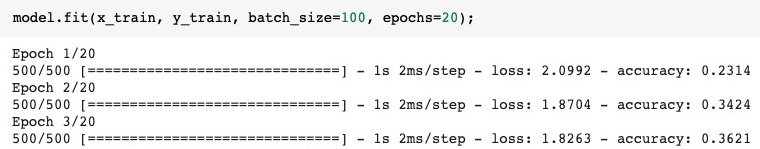
\includegraphics[width=\textwidth]{training-start.jpg}
        \begin{center}
            $\vdots$
        \end{center}
        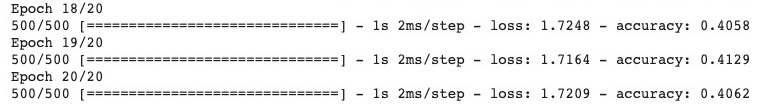
\includegraphics[width=\textwidth]{training-end.jpg}
        
        \bigskip
        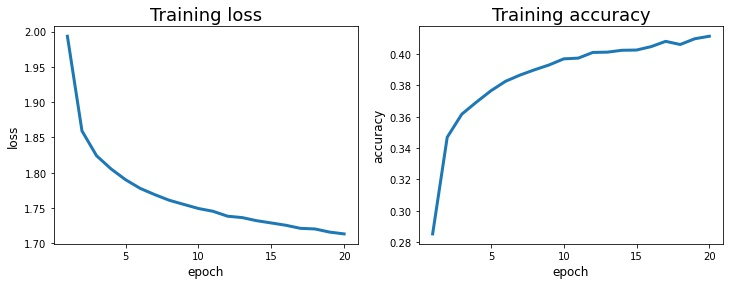
\includegraphics[width=\textwidth]{loss-accuracy.jpg}
    
    \end{frame}
    
\end{document}
